\documentclass[a4paper,11pt,pdftex]{article}

\usepackage[utf8]{inputenc}
%\usepackage[magyar]{babel} %needed in Hungarian reports
\usepackage{fancyhdr} %for the nice header
\usepackage{graphicx} %grapics input
\usepackage{tikz} %tikz figures

\usepackage{amsmath}
\usepackage{amsthm}
\usepackage{amssymb}


\usepackage[a4paper,left=2.5cm,right=2.5cm,top=2.5cm,bottom=2.5cm,pdftex]{geometry} %margins

\usepackage{color}
\usepackage{url}
\usepackage{hyperref} %links
\hypersetup{
colorlinks=true,
linkcolor=blue,
urlcolor=blue,
citecolor=red
}

\rhead{NLDC II.}
\lhead{Homework 5}
\chead{B. Kaszas}

\setlength{\parskip}{0.5em}
\setlength{\parindent}{0em}

\title{Nonlinear Dynamics and Chaos II. \\ Homework 5}
\author{Kaszás Bálint}
\date{\today}

\begin{document}
\pagestyle{fancy}

\maketitle


\section*{Exercise 1}
Consider the slowly forced pendulum with viscous damping

\begin{equation*}
    \label{eq1}\ddot{\varphi} + k\dot{\varphi} + \sin \varphi = F_0 \sin (\varepsilon t)
\end{equation*}
$k>0$ is the damping coefficient, $F_0<1$ and $0<\varepsilon \ll 1$. 

\emph{Solution}

To write the system in first order, autonomous form, let $v = \dot{\varphi}$ and $\psi = \varepsilon t$. 

\begin{align*}
    \dot{\varphi} & = v \\
    \dot{v} & = -k v - \sin \varphi + F_0 \sin \psi \\
    \dot{\psi} &= \varepsilon.
\end{align*}
This is a problem that has separated timescales, and can be viewed as a singularly perturbed problem, on the fast timescale. Here, $\varphi$ and $v$ are the fast variables, while $\psi$ is the slow variable. Setting $\varepsilon = 0$, we get the fast subsystem:

\begin{align*}
    \dot{\varphi} & = v \\
    \dot{v} & = -k v - \sin \varphi + F_0 \sin \psi \\
    \dot{\psi} &= 0.
\end{align*}

To obtain the critical manifold $C_0$, we look for fixed points of this system. Because of the first equation, we must have $v=0$. Substituting it into the second equation, we get
\begin{equation*}
    0 = -\sin \varphi + F_0 \sin \psi.
\end{equation*}

Since $F_0<1$, this has has two solutions for all $\psi$. 
\begin{equation}
\label{root1}
    \varphi_1(\psi) = \text{arcsin}(F_0 \sin \psi)
\end{equation}

or
\begin{equation}
\label{root2}
    \varphi_2(\psi) = -\text{arcsin}(F_0 \sin \psi) + \pi.
\end{equation}

The extended phase space is spanned by the variables $(\varphi, v, \psi)$. But since $\varphi$ and $\psi$ are cyclic, the phase space can be viewed as the manifold $S^1 \times S^1 \times \mathbb{R}  \sim T^2 \times \mathbb{R}$. Because we were able to write the fixed points as a graph over $\psi$, the critical manifold is

$$
C_0 = \{ (\varphi, \psi, v) \in S^1 \times S^1 \times \mathbb{R} : v = 0, \varphi = \text{arcsin}(F_0 \sin \psi), \varphi = -\text{arcsin}(F_0 \sin \psi) + \pi
\}.
$$
This is a union of two disjoint curves. The normal hyperbolicity of the manifold depends on the hyperbolicity of the fixed points, in the fast subsystem. 

\begin{align*}
    \frac{d}{dt}\begin{bmatrix}
    \varphi \\
    v 
    \end{bmatrix} &= \begin{bmatrix} 
     v \\
    -k v - \sin \varphi + F_0 \sin \psi 
    \end{bmatrix} := f(\varphi, v) \\
    \dot{\psi} &= 0 
\end{align*}
The Jacobian matrix $D_{\varphi, v} f(\varphi,v)$ is
$$
D_{\varphi, v} f(\varphi,v) = \begin{bmatrix} 
0 & 1 \\
-\cos \varphi & -k
\end{bmatrix},
$$

which we have to evaluate at the points (\ref{root1}) and (\ref{root2}) and look for its eigenvalues. The characteristic polynomial is 
$$
\lambda^2  + k \lambda + \cos \varphi_{1,2}(\psi) = 0,
$$
with roots

\begin{equation}
\label{eigen}
    \lambda_{\pm} =  -\frac{k}{2} \pm \sqrt{\frac{k^2}{4} - \cos \varphi_{1,2}(\psi)}.
\end{equation}

Here, by substituting (\ref{root1}) and (\ref{root2}), we get
$$
\cos \varphi_1 = \cos (\text{arcsin}(F_0\sin \psi) ) = \sqrt{1 - F_0^2 \sin^2 \psi} >0
$$
and
$$
\cos \varphi_2 = \cos (-\text{arcsin}(F_0\sin \psi)+\pi) = -\cos( \text{arcsin}(F_0\sin \psi)) = - \sqrt{1 - F_0^2 \sin^2 \psi} <0,
$$
by the properties $\cos(\pi - \theta) = - \cos \theta$ and $\cos(\text{arcsin}(x)) = \sqrt{1-x^2}$.
Evaluating (\ref{eigen}) at these points, we see that in case of the first root, $\varphi_1$, the square root is strictly smaller than $k/2$, both eigenvalues are negative.
At the root $\varphi_2$, the square root is strictly larger than $k/2$, which means $\lambda_+$ becomes positive. 

Both fixed-curves $\varphi_{1,2}(\psi)$ of the fast subsystem are hyperbolic, $\varphi_1$ is asymptotically stable and $\varphi_2$ is unstable. This means that the critical manifold $C_0$ is a normally hyperbolic invariant manifold. 

The full system is an $\varepsilon$-size perturbation to the fast subsystem, and we can conclude that there exists a normally hyperbolic invariant manifold $C_\varepsilon$, $\varepsilon$ close to $C_0$, which is the slow manifold. 

The full extended phase space $S^1 \times S^1 \times \mathbb{R}$, can be viewed as the product of a 2-torus and the real line. The critical manifold (and $\varepsilon$ close to it, the slow manifold) then, is an union of two curves, that run on the 2-torus, corresponding to the section $v=0$. 

We can represent this torus as an embedded submanifold of $\mathbb{R}^3$, parametrized by $(\varphi, \psi)$. 

\begin{figure}[h]
    \centering
    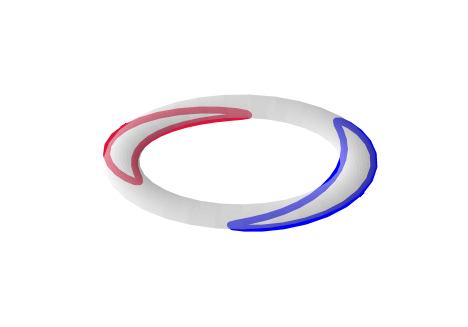
\includegraphics[width = 0.5\textwidth]{torus.png}
    \caption{Slow manifold of the slowly forced pendulum. The torus shown is the $v=0$ section of phase space. The colored curves make up the slow manifold, the blue one is $\varphi_1(\psi)$ and the red one is $\varphi_2(\psi)$. }
    \label{fig:t}
\end{figure}
The slow manifold is shown in Fig. \ref{fig:t}. The red curve is the unstable part of $C_\varepsilon$ and the blue one is the stable part. 
They trace out closed curves, $\varphi_1$ oscillating between $-\text{arcsin}(F_0)$ and $\text{arcsin}(F_0)$ and $\varphi_2$ between $\pi + \text{arcsin}(F_0)$ and $\pi-\text{arcsin}(F_0)$. 
In the extended phase space, $S^1 \times S^1 \times \mathbb{R}$ (the torus shown is just a submanifold of this), 
the curve $\varphi_2$ has a local stable manifold and an unstable manifold. Trajectories in the stable manifold would converge to $\varphi_2$, while all other nearby trajectories would converge to $\varphi_1$. 

\section*{Exercise 2}
Stommel's model for the Thermohaline circulation is 
\begin{align}
   \label{eqstomm}
    \dot{x} &= -\frac{1}{\tau_x}(x-1) + \frac{1}{\tau_y}x[1+\eta^2(x-y)^2] \\
    \dot{y} & = \frac{\mu}{\tau_y} - \frac{1}{\tau_y}y[1+\eta^2(x-y)^2].
\end{align}
The variables are $x,y$, where $x(t)$ is the temperature-gradient and $y(t)$ is the salinity gradient. The parameter $\mu$ is the freshwater flux, $\eta$ is the nonlinear coupling constant. The relaxation times for the two processes are $\tau_x$ and $\tau_y$, which satisfy $\tau_x/\tau_y = \varepsilon \ll 1$.

(a) Show that Stommel's model has a globally attracting slow manifold that governs the asymptotic behavior of THC. Find a leading order approximation to this manifold. 

\emph{Solution}

Introducing the new timescale $s=t\tau_y$, $d/dt = 1/\tau_y d/ds$:
\begin{align*}
    \frac{1}{\tau_y}\frac{dx}{ds} &= -\frac{1}{\tau_x}(x-1) + \frac{1}{\tau_y}x[1+\eta^2(x-y)^2] \\
    \frac{1}{\tau_y}\frac{dy}{ds} & = \frac{\mu}{\tau_y} - \frac{1}{\tau_y}y[1+\eta^2(x-y)^2].
\end{align*}
Using the definition of $\varepsilon$, we have the singular perturbation problem, with $x$ the fast variable and $y$ the slow variable. 
\begin{align}
\label{eqfast1}
    \varepsilon\frac{dx}{ds} &= -(x-1) + \varepsilon x[1+\eta^2(x-y)^2]:=f(x,y,\varepsilon) \\
    \label{eqfast2}
    \frac{dy}{ds} & = \mu - y[1+\eta^2(x-y)^2] :=g(x,y).
\end{align}
Switching timescales again, by $s=\varepsilon \tau$ and denoting the differentiation with respect to $\tau$, by $(\cdot)'$ 
\begin{align*}
    x' &= -(x-1) + \varepsilon x[1+\eta^2(x-y)^2] \\
    y' & = \varepsilon\left(\mu - y[1+\eta^2(x-y)^2]\right).
\end{align*}
Setting $\varepsilon = 0$, we get the fast subsystem:
$$
x' = -(x-1) 
$$
and $y' = 0$.

We look for the fixed point of this subsystem, which is $x=1$, for any $y$, which means we can write the critical manifold as
\begin{equation}
    C_0 = \{ (x,y): x = 1\}. 
\end{equation}
The stability of the critical manifold depends on the stability of the fixed point $x=1$ in the fast subsystem. Since 

$$
\frac{d}{dx}f(x,y,0) = -1
$$
this fixed point is hyperbolic and also attracting with a rate $e^{-\tau}$. Because of this, the critical manifold $C_0$ is a normally attracting invariant manifold for the system, for $\varepsilon = 0$. 

As a result of Fenichel's theorem, we conclude that for small enough $\varepsilon$, there is a normally attracting invariant manifold $C_\varepsilon$ for the system (\ref{eqstomm}), which is $O(\varepsilon)$ close to $C_0$. This is the slow manifold, which we can represent as a graph

$$
C_\varepsilon = \{ (x,y): x = \varphi(y,\varepsilon)\}.
$$
Because of the smoothness properties, we can expand it in terms of $\varepsilon$: $x = \varphi(y,\varepsilon) = \varphi_0(y) + \varepsilon \varphi_1(y) + O(\varepsilon^2) = 1+\varphi_1(y)+O(y^2)$.


On one hand, on the manifold we have $x = \varphi(y,\varepsilon)$, which we can differentiate with respect to $\tau$.
\begin{equation}
    \label{eq11}
    x' = \frac{d \varphi}{d y} y' = \varepsilon^2 \frac{d\varphi_1(y)}{dy}\left( \mu- y -y\eta^2(1+\varepsilon\varphi_1(y) -y)^2\right) = O(\varepsilon^2).
\end{equation}

On the other hand, we can use the $x'$ equation restricted to the manifold. 
\begin{align*}
        \label{eq22}
    x' &= f(\varphi(y,\varepsilon),y,\varepsilon) = -\varepsilon \varphi_1(y) + \varepsilon x[1+\eta^2(x-y)^2]= \\
    &= -(x-1) + \varepsilon x[1+\eta^2(x^2-2xy + y^2)] = \\
    &= -\varepsilon\varphi_1(y) + \varepsilon + \varepsilon \eta^2(1-2y +y^2) +O(\varepsilon^2).
\end{align*}
For the manifold to be invariant, these two expressions must match in all orders of $\varepsilon$. Since in (\ref{eq11}), there were no order $\varepsilon$ terms, we must get 0 for the coefficient of the $O(\varepsilon)$ term in the latter expression. This means

$$
\varphi_1(y)= 1 + \eta^2(1-y)^2.
$$

To leading-order, the slow manifold is described by the graph $x = 1 + \varepsilon(1+\eta^2(1-y)^2)$.

(b) Compute the leading-order reduced flow on the slow manifold. Determine qualitatively the possible dynamical behaviors on the slow manifold as the parameters $\mu$ and $\eta$ are varied.

\emph{Solution}

To derive the reduced order flow, we Taylor-expand the equation governing the slow variable (on the original timescale, $s$):

\begin{equation*}
    g(x,y) = g(\varphi_0(y), y) + \varepsilon\left(\frac{d g}{dx}|_{(\varphi_0(y),y)}\right)\varphi_1(y) + O(\varepsilon^2)
\end{equation*}
From (\ref{eqfast2}), $g(x,y)= \mu - y[1+\eta^2(x-y)^2]$
$$
g(x,y) = \mu - y[1+\eta^2(1-y)^2] -2 \varepsilon\varphi_1(y)\eta^2y(1-y) + O(\varepsilon^2)
$$
Plugging in the expression for $\varphi_1$, we have

$$
g(x,y) = \mu - y[1+\eta^2(1-y)^2] -2 \varepsilon(1 + \eta^4y(1-y)^3) + O(\varepsilon^2)
$$
Keeping only the leading order term, we get the reduced dynamics on the slow manifold
$$
\frac{dy}{ds} = \mu - y[1+\eta^2(1-y)^2].
$$

On the slow manifold, the long time behavior of solutions is dictated by the fixed points. They are the roots of the right hand side:

$$
\mu = y[1+\eta^2(1-y)^2]
$$

The graph of these functions are shown in Fig. \ref{fig:c}. The fixed points of the system are given by the intersection points. 
\begin{figure}[h!]
    \centering
    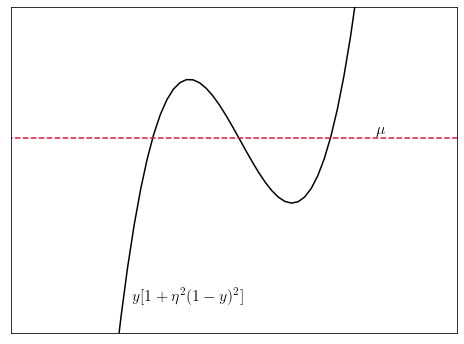
\includegraphics[width = 0.4\textwidth]{cubic.png}
    \caption{Graphs of the functions $f(y) = \mu$ and $f(y)= y[1+\eta^2(1-y)^2]$.}
    \label{fig:c}
\end{figure}
To see the effect of the parameters, note that the shape of the cubic function is only governed by $\eta$. It can have at most two critical points, one minimum and one maximum. These are:
$$
\frac{d}{dy}y[1+\eta^2(1-y)^2] =0
$$

$$
1 + \eta^2(1-y)^2 - 2y \eta^2 (1-y) = 0
$$

$$
3\eta^2 y^2 - 4y\eta^2 +1 + \eta^2 = 0.
$$
This equation has two roots (the minimum and maximum of the cubic function) if 
$$
16\eta^4 - 12\eta^2(1+\eta^2) > 0,
$$
or $\eta^2 > 3$. In this case, the intersection of this graph with $y=\mu$ can give 1, 2 or 3 values. If $y$ is smaller or larger than any of the critical values of the graph, there is only one solution. In these cases the right hand side of the system $\mu - y[1+\eta^2(1-y)^2]$ changes sign at the fixed points, and they are stable. 

When $\mu$ reaches (one of) the critical values, a new fixed point appears in a bifurcation.

When $\mu$ is between the critical values, we have 3 fixed points, two stable and one unstable. 

When the above discriminant is 0, at $\eta^2 = 3$,  the cubic graph has only one critical point, and for all values of $\mu$ we only have one fixed point. This fixed point is stable. 
\end{document}
